\apendice{Documentación técnica de programación}

\section{Introducción}
En este apartado se especificará la estructura de directorios de la aplicación y la instalación de materiales y recursos como una herramienta para programadores.

Para ello, se separará en tres secciones:
\begin{itemize}
    \item Estructura del repositorio: estructura de carpetas en git de la aplicación.
    \item Instalación, compilación y requisitos de entorno: explica cómo instalar y arrancar la aplicación y los requisitos para ello.
    \item Servicio web: se explicará la importación del despliegue a través de una máquina virtual para su posterior uso, así como la configuración de las instancias del servidor.
\end{itemize}

\section{Estructura del repositorio}
El repositorio en Git cuenta con la siguiente distribución principal:
\begin{itemize}
    \item \textbf{Directorios}: carpetas contenedoras de los archivos del proyecto.
    \item \textbf{Ramas o ``branches''}: distintas versiones del código de la aplicación en las distintas fases.
    \item \textbf{Issues}: tareas asignadas del proyecto.
    \item \textbf{Milestones}: hilo de proyecto que distribuye las tareas o issues. Cada milestone representa una fase o subfase del proyecto, que coincide con las etapas del modelo de la metodología usada y explicada previamente.
\end{itemize}

\subsection{Directorios}
Esta parte representa el contenido del proyecto en su totalidad. Las diferentes carpetas que se incluyen en el proyecto son:
\begin{itemize}
    \item \textbf{CSACVM}: es el núcleo y carpeta contenedora principal del proyecto. La estructura de esta carpeta se ha explicado previamente en el apartado de diseño, ya que es la que forma la aplicación con el resto de dependencias, librerías y subproyectos.
    \item \textbf{Documentación}: en esta carpeta se guarda toda la documentación del proyecto, como por ejemplo la memoria, los anexos, las imágenes utilizadas, etc.
    \item \textbf{DespliegueWeb}: carpeta contenedora de los archivos para la instalación del despliegue de la web con la máquina virtual.
    \item \textbf{ScriptsDB}: en esta carpeta se guardan los scripts de los datos de la base de datos que se utiliza por si se quiere instalar de forma local.
\end{itemize}

\subsection{Ramas, issues y milestones}
Las issues son las tareas asignadas del proyecto con las que se controlan los cambios de funcionalidad de este, tanto en código como a la hora de añadir/generar archivos, carpetas, estructura de proyecto o librerías.

Todas las issues tienen asignadas una milestone, ya que esta es la forma óptima de separar funcionalidad a través de las distintas fases del proyecto. Además de esto, las issues tienen labels que se han ido añadiendo y quitando durante su desarrollo.

Las labels más utilizadas han sido:
\begin{itemize}
\tightlist
    \item En proceso: issues que se encuentran en desarrollo en ese momento.
    \item \emph{Bug}: issues con partes que tienen errores que se intentan corregir.
    \item Documentation: issues para añadir o modificar los archivos de la documentación del proyecto.
    \item \emph{WontFix}: issues que se habían creado para cierto propósito que no se van a corregir o descartes de funcionalidad.
\end{itemize}

Como se ha explicado, las milestones forman cada distinta fase o etapa del flujo del desarrollo del proyecto. Cada milestone tiene:
\begin{itemize}
\tightlist
    \item Issues asignadas con la funcionalidad de esa etapa.
    \item Descripción de la fase y de las tareas que se llevarán a cabo.
\end{itemize}

Las milestones y las ramas también guardan relación, pues estas últimas guardan la versión del código en cada fase. Como diferencia, las milestones a veces dividen una rama o fase en varios subapartados.

Para dar un ejemplo del caso anterior, podemos tener una milestone de la fase 3 con varios subapartados (3.1, 3.2, 3.x...) pero todo se realiza en solamente una rama (rama para la fase 3).

\section{Instalación, compilación y ejecución del proyecto}
En esta parte del manual de programador, se va a explicar cómo realizar la instalación del proyecto y los requisitos para ello.

\subsection{Requisitos}
En primer lugar, necesitamos saber en qué entorno se va a utilizar el proyecto para saber qué herramientas debemos obtener antes de la clonación del proyecto. Para ello, necesitaremos:
\begin{itemize}
    \item \textbf{Entorno (IDE)}: el entorno que se utiliza es Visual Studio 2022, en mi caso personal se utiliza la versión ``Community'' (es gratuito) aunque tanto las versiones de ``Enterprise'' como ``Professional'' (ambas de pago con licencia) son igual de válidas 
    (a gusto del usuario).
    \item \textbf{SSMS}: Sql Management Studio 18 es el gestor de bases de datos que se utilizado para la realización del proyecto.
    \item \textbf{Git}: git es el controlador de versiones y a parte es una herramienta que permite ejecutar funciones para git. No es extremadamente necesario porque la clonación se hará a través de Visual Studio, pero también se explicará su uso a través de la consola de comandos.
\end{itemize}

Para la instalación de Visual Studio, se tienen que instalar ciertos paquetes:
\begin{itemize}
\tightlist
    \item Desarrollo de ASP.NET y web.
    \item Desarrollo de escritorio de \emph{.NET}.
    \item Desarrollo de \emph{Node.js}.
    \item Herramientas de \emph{EntityFramework} 6 y \emph{.NET WebAssembly}.
    \item SQL Server Express 2019 LocalDB.
    \item Paquetes de compatibilidad de \emph{.NET Framework} (del 4.6 al 4.8).
    \item ASP.NET MVC 4.
\end{itemize}

\subsection{Instalación}
Una vez tengamos las herramientas anteriores en nuestro sistema, daremos paso a la clonación del proyecto, importación de la base de datos y ciertos apuntes para la compilación que pueden servir a modo de ayuda.

\subsubsection{Clonación del repositorio con Visual Studio}
Es posible que nada más arrancar Visual Studio nos muestre una ventana para crear un nuevo proyecto o clonar uno existente.

\begin{figure}
    \centering
    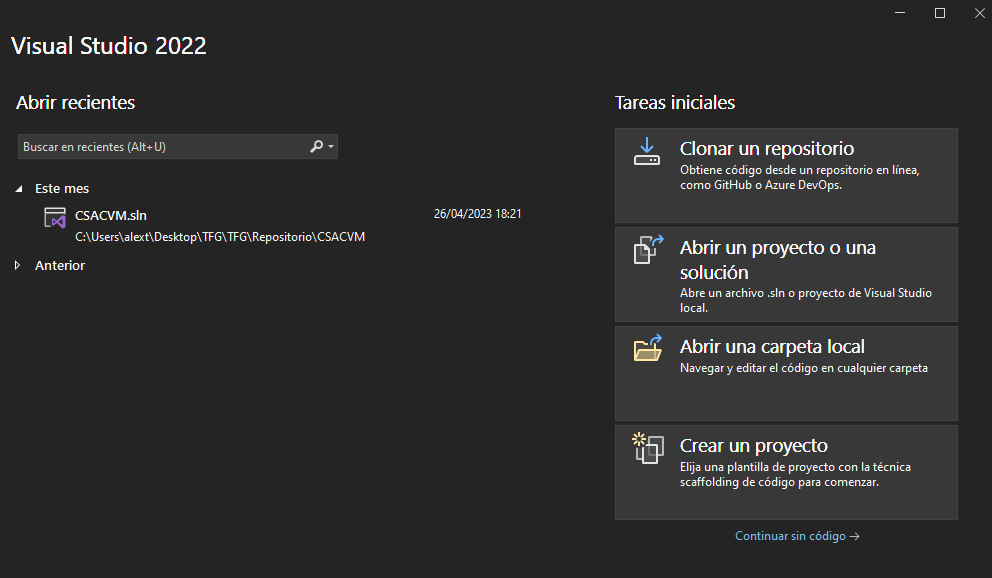
\includegraphics[width=\linewidth]{img/ManualProgramador/ClonacionP1.png}
    \caption{Clonación repositorio paso 1}
    
\end{figure}

Para clonar el repositorio, simplemente necesitamos copiar la url del repositorio en Github y especificar la carpeta donde va a estar nuestro proyecto en el sistema.

\begin{figure}
    \centering
    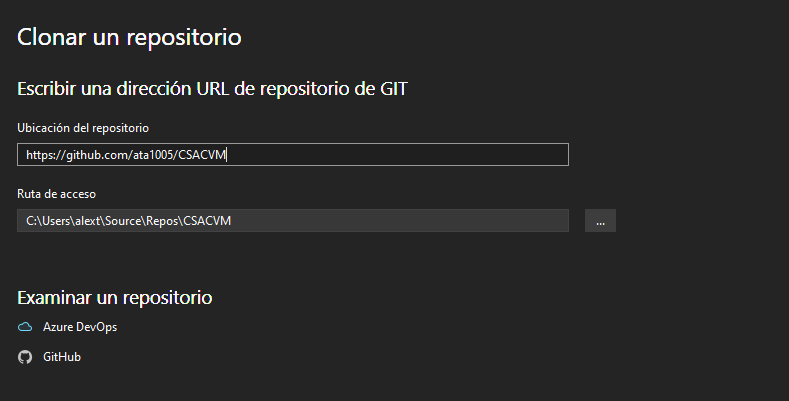
\includegraphics[width=\linewidth]{img/ManualProgramador/ClonacionP2.png}
    \caption{Clonación repositorio paso 2.1}
    
\end{figure}

También podemos añadir nuestra cuenta de Github y seleccionar el repositorio de forma manual.

\begin{figure}
    \centering
    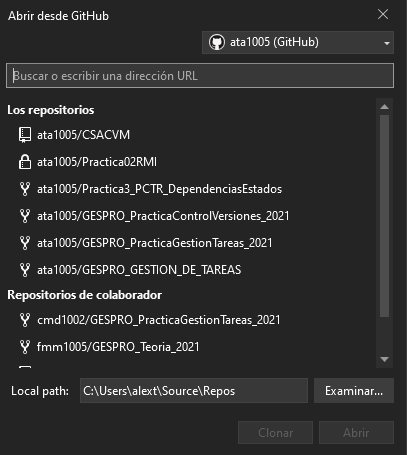
\includegraphics[width=\linewidth]{img/ManualProgramador/ClonacionP3.png}
    \caption{Clonación repositorio paso 2.2}
    
\end{figure}

\subsubsection{Clonación del repositorio con Git}
Para clonar el repositorio también podemos utilizar la consola de comandos de Git. En esta caso seguiremos los siguientes pasos:
\begin{itemize}
    \item Creamos una carpeta o directorio donde guardar el proyecto.
    \item Dentro de esa carpeta, abrimos la consola de Git (o en cualquier otro lado pero accediendo después a esta carpeta).
    \item Una vez dentro de la consola, escribimos el comando ``git clone'' seguido de la url que hemos copiado del repositorio del proyecto en github.
\end{itemize}

Una vez hecho esto ya solo queda entrar en Visual Studio y seleccionar nuestro proyecto entrando en la solución de la carpeta que hemos elegido.

\subsubsection{Añadir base de datos}
Como se ha indicado, los scripts para añadir la base de datos se encuentran en el repositorio de github. Una vez se haya instalado el SQL Management Studio, lo abrimos y seleccionamos el entorno o conexión en la que queremos conectarnos.

Por defecto se selecciona el ``localDB'' que es el host local del servidor de nuestro sistema, que se conecta a través de dos perfiles, dependiendo del sistema:
\begin{itemize}
\tightlist
    \item La cadena de conexión es solamente un punto (``.'').
    \item La cadena de conexión es: ``(localdb)\textbackslash MSSQLLocalDB''.
\end{itemize}

De todas maneras, si tenemos otro servidor en nuestro SQL en el que queramos añadir la base de datos, también lo podemos hacer.

Ahora solo nos queda importar la base de datos. Para ello, abrimos con el SQL Management Studio el script descargado y lo ejecutamos. Como el script que se incluye ya genera tanto la base de datos como las tablas y sus datos, no tendremos que hacer nada más.

\subsubsection{Configuración y compilación}
Si el servidor de base de datos fuera distinto al LocalDB, tendríamos que cambiar la cadena de conexión. Para ello debemos acceder al ``appsettings.json'' del proyecto principal, y cambiar el atributo de ``ConnectionStrings'', añadiendo en esa línea el enlace al servidor en el que se ha instalado la base de datos.

\begin{figure}[h]
    \centering
    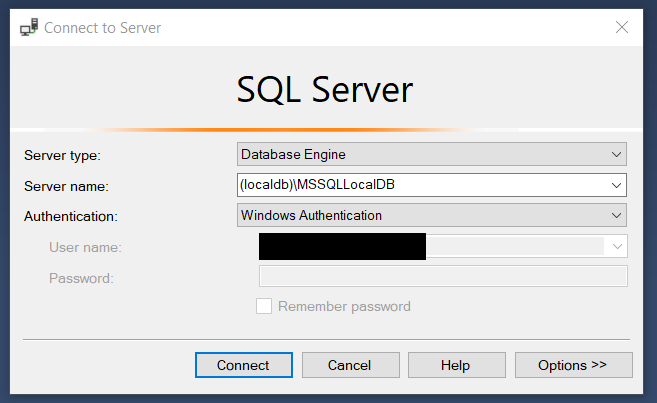
\includegraphics[width=\linewidth]{img/ManualProgramador/SQLConnect.png}
    \caption{Conexión en el SQL Management Studio}
\end{figure}
\begin{figure}
    \centering
    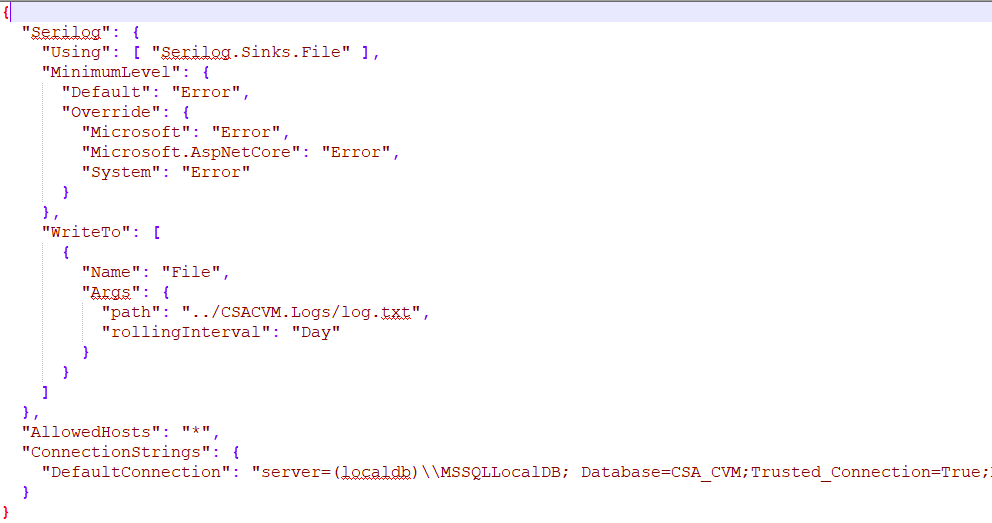
\includegraphics[width=\linewidth]{img/ManualProgramador/Settings.png}
    \caption{Cadena de conexión Programa - SQL Server}
    
\end{figure}

\newpage
Para compilar y ejecutar la aplicación, tenemos la configuración inicial. No obstante, podemos cambiar tanto el inicializador como el navegador que queramos utilizar.
\begin{figure}
    \centering
    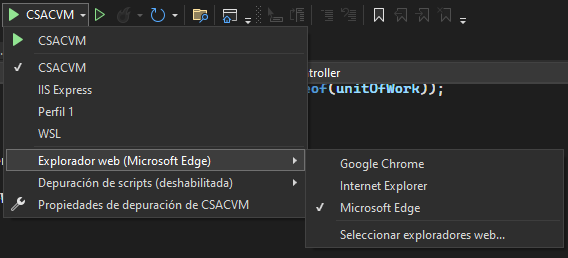
\includegraphics[width=\linewidth]{img/ManualProgramador/depuracion.png}
    \caption{Compilación y ejecución de la aplicación}
    
\end{figure}

\newpage
\section{Servicio web con máquina virtual}
Como se ha mencionado previamente, el despliegue del servidor web se realiza a través de una
máquina virtual de Windows 10.

Dentro de la máquina tenemos varias partes:
\begin{itemize}
\tightlist
    \item SQL Server: se instancia un servidor de base de datos en el que se aloja la database.
    \item IIS Express: configurador de los servicios web. En él se crea una instancia del proyecto, en el que se indica a qué directorio se apunta para obtener la configuración de la aplicación y lanzarla.
    \item Directorio web: en él guardamos los archivos de la publicación del proyecto.
\end{itemize}

\subsection{Configuración de los servicios}
Para crear la instancia de la web utilizaremos el IIS Manager.
\begin{figure}[H]
    \centering
    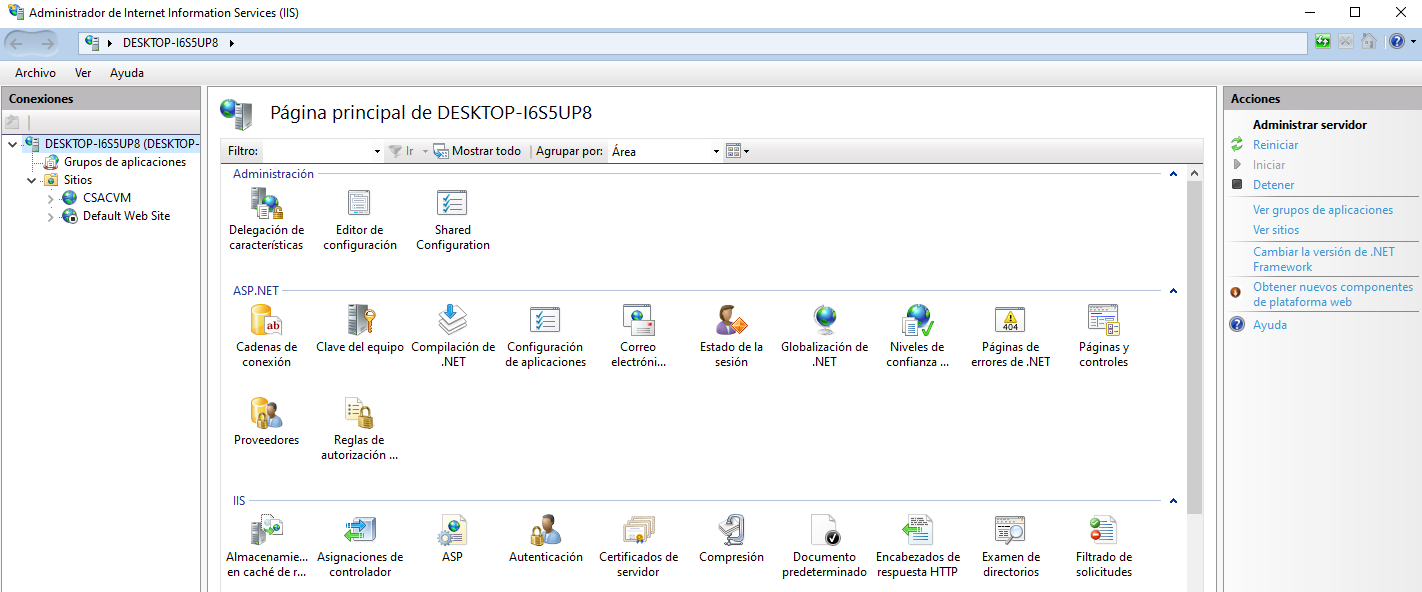
\includegraphics[width=\linewidth]{img/ManualProgramador/Despliegue01.png}
    \caption{IIS Manager - Página principal}
    
\end{figure}

Esta es la pantalla principal del configurador, en él se crean/instancian las aplicaciones web.
Como vemos en la parte de la izquierda, podemos configurar los grupos de aplicaciones y sus respectivos sitios web. 

\begin{figure}
    \centering
    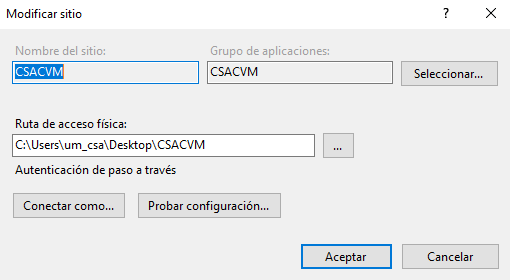
\includegraphics[width=\linewidth]{img/ManualProgramador/Despliegue02.png}
    \caption{IIS Manager - Configuración básica}
    \label{iisBasica}
\end{figure}

En la configuración básica (fig. \ref{iisBasica}), podemos indicar el nombre y la ruta de acceso directa al directorio donde se publica la aplicación, para que pueda obtener los archivos de configuración y desplegar la web.

\begin{figure}
    \centering
    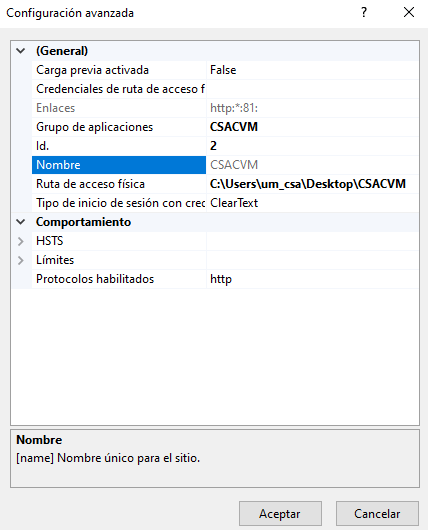
\includegraphics[width=\linewidth]{img/ManualProgramador/Despliegue03.png}
    \caption{IIS Manager - Configuración avanzada}
    \label{iisAvanzada}
\end{figure}

En la configuración avanzada (fig. \ref{iisAvanzada}) podemos indicar los hosts y los límites que vienen configurados. Normalmente estos atributos permanecen por defecto, pero se pueden personalizar. También es importante indicar el puerto en el que se despliega la web. Esto es importante porque el puerto es único para cada una de las páginas web que se van a alojar en el IIS.

Como la aplicación se ha desarrollado en Core, también ha hecho falta instalar un \href{https://learn.microsoft.com/en-us/aspnet/core/host-and-deploy/iis/hosting-bundle?view=aspnetcore-7.0}{``hosting bundle''}\footnote{Hosting Bundle para ASPNET Core: https://learn.microsoft.com/en-us/aspnet/core/host-and-deploy/iis/hosting-bundle?view=aspnetcore-7.0} que permite la ejecución de la web.

Finalmente, para la comunicación con la base de datos, se ha creado un usuario específico y se ha añadido directamente a la cadena de conexión de la aplicación, para que se pueda conectar con usuario y contraseña al servidor de base de datos.